
\section{RBA XML}
\label{sec:rba_xml}

\paragraph{Metabolism file}
\begin{figure}[ht]
  \centering
  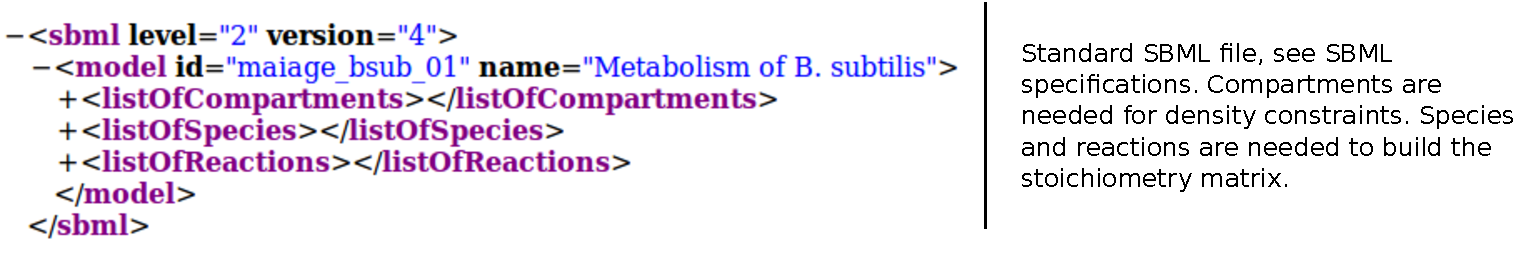
\includegraphics[width=\linewidth]{metabolism}
  \caption{Metabolism file is a standard SBML file.}
  \label{fig:metabolism}
\end{figure}
The metabolism file is a standard SBML file~\reffigp{fig:metabolism}. It contains information about cell compartments, metabolite species and metabolism reactions. Concentration of external metabolites are defined in the species section.

\paragraph{Parameter file}
\begin{figure}[ht]
  \centering
  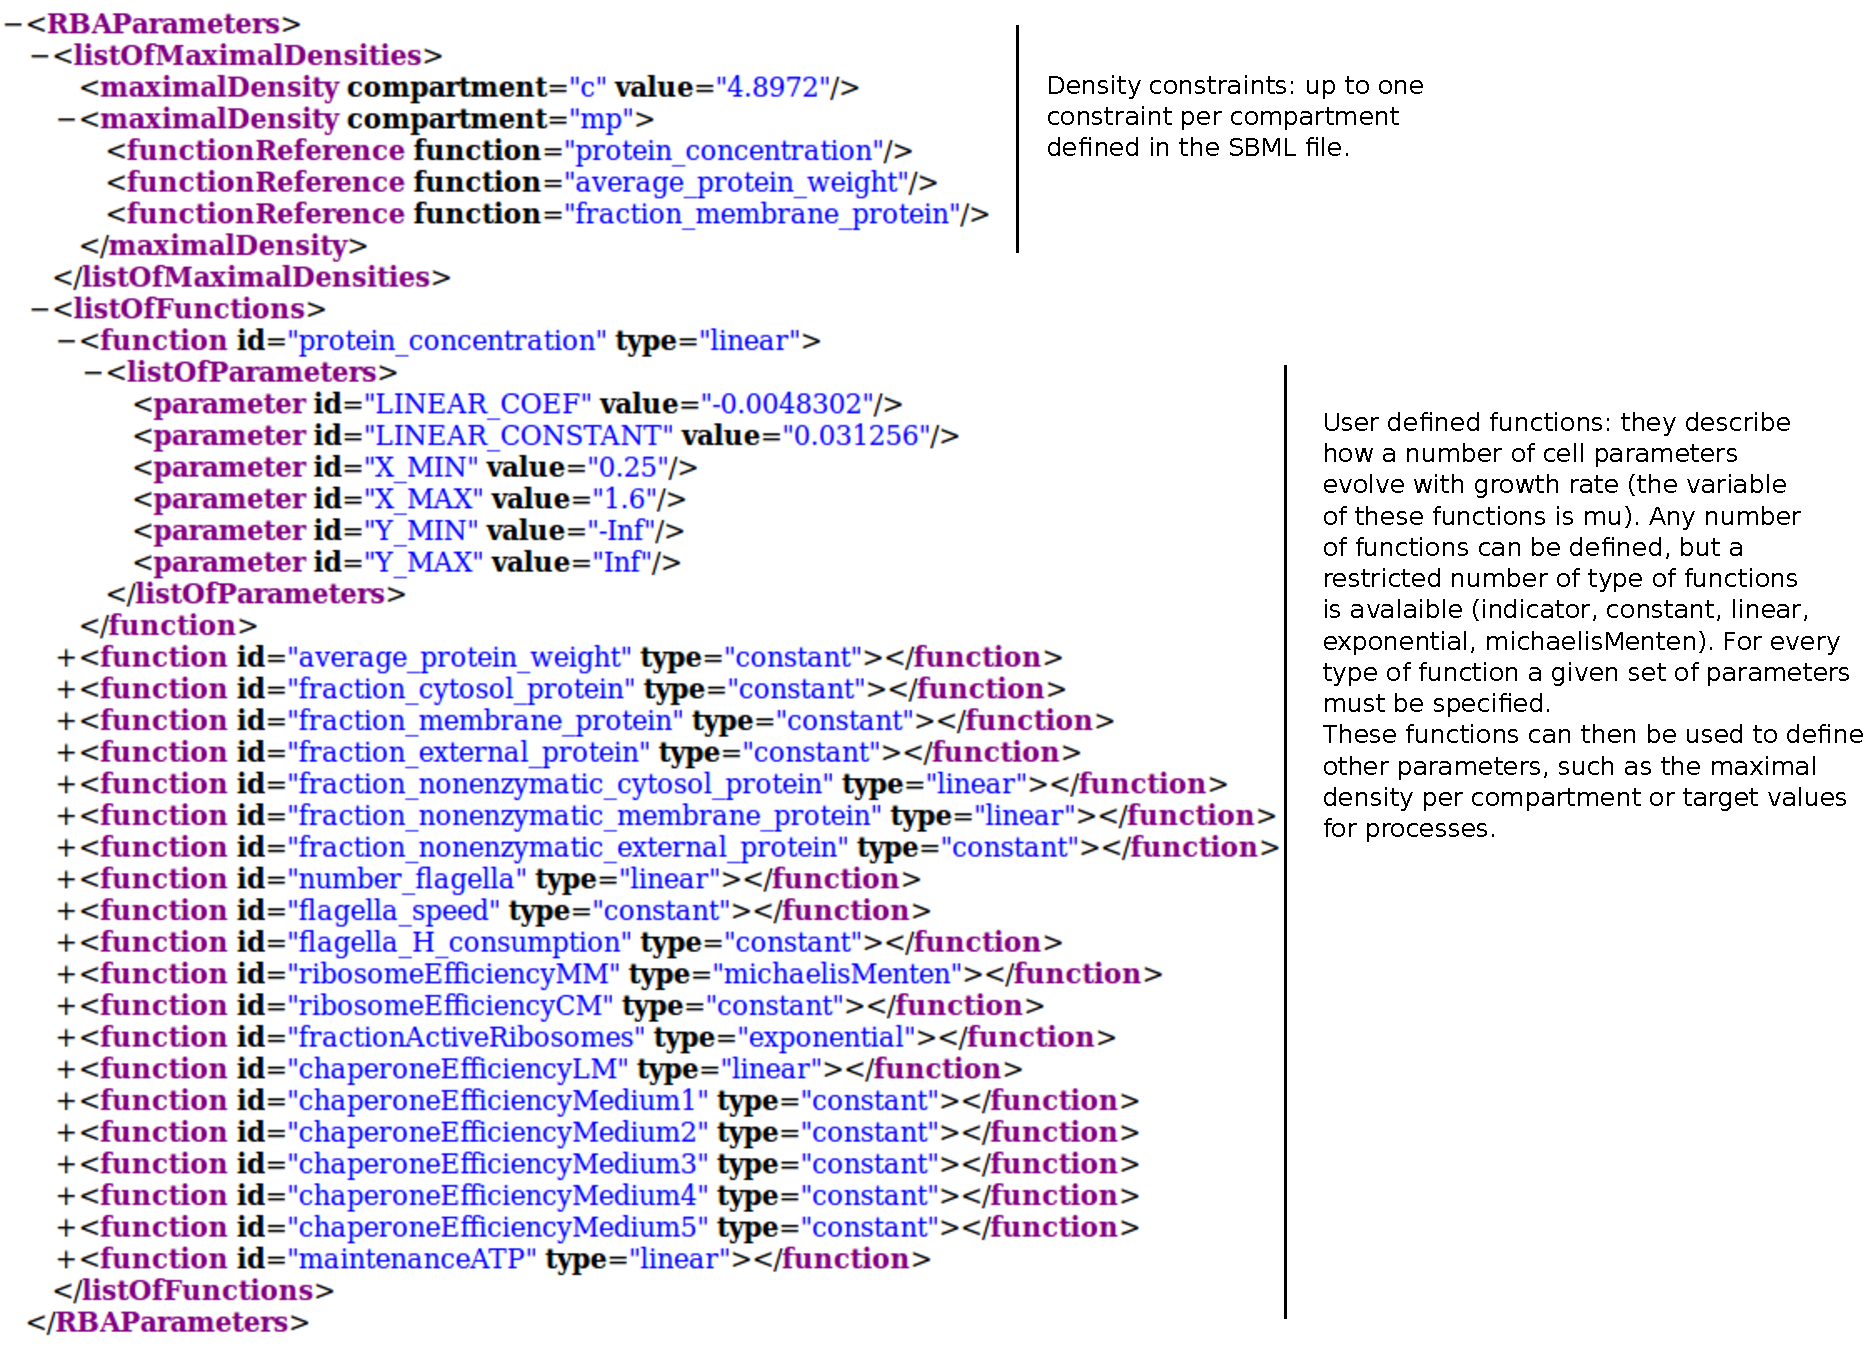
\includegraphics[width=\linewidth]{parameters}
  \caption{Structure of the parameter file used by RBA.}
  \label{fig:parameters}
\end{figure}
The parameter file is an XML file composed of two subsections~\reffigp{fig:parameters}. \texttt{listOfMaximalDensities} contains density constraints. \texttt{listOfFunctions} contains user-defined functions that can be used to set $\mu$-dependent maximal densities or $\mu$-dependent process targets (see below).

\paragraph{Macromolecule files}
\begin{figure}[ht]
  \centering
  \includegraphics[width=\linewidth]{proteins}
  \includegraphics[width=\linewidth]{rnadna}
  \caption{Structure of protein, RNA and DNA file.}
  \label{fig:proteins}
\end{figure}
Currently, RBA defines three sets of macromolecules: proteins, RNAs and DNA. One XML file is created for each set~\reffigp{fig:proteins}. All macromolecules have a \texttt{listOfComponents} describing the building blocks used to produce them (\textit{e.g.} amino acids, vitamins and ions for proteins). Then a \texttt{listOfSpecies} contains all molecules of the set, including their description in terms of components. Additionally, proteins have a \texttt{listOfEfficiencyFunctions} that lists efficiency models for enzymes. Enzymes contain an \texttt{enzymaticActivity} structure that defines the reaction they catalyze and the parameters for the efficiency models. Finally, transporters have a \texttt{transporterEfficiency} that modulates the enzymatic activity depending on substrate and cofactor availability.

\paragraph{Process file}
\begin{figure}[ht]
  \centering
  \includegraphics[width=\linewidth]{processes}
  \caption{Structure of process file.}
  \label{fig:processes}
\end{figure}
The process file is an XML file containing a \texttt{listOfProcesses} and a \texttt{listOfComponentMaps}. Each \texttt{process} can contain up to 3 subsections. The \texttt{capacityConstraint} defines a machinery used by the process that has a limited capacity. The \texttt{operatingCosts} defines which macromolecules the process produces/degrades/modifies and the cost associated with these operations. The \texttt{targets} are set fluxes that a process must maintain in order for the cell to work properly. Target fluxes can apply to metabolites (\texttt{targetValue}) and reactions (\texttt{targetReaction}). Target fluxes scale with $\mu$ if they contribute to \texttt{dilution\_compensation} or if they are defined using a $\mu$-dependent user-function. Finally \texttt{componentMaps} are used to compute the costs in the \texttt{operatingCosts} section.
